%\vspace*{-0.2cm}
\section{Implementation}
\label{sec:impl}

We have implemented our consistent hashing with random load update (RLU) policy and other load-balancing policies in OpenWhisk, a popular FaaS system.
Our changes amount to more than 1,700 lines of code across many OpenWhisk components, but are primarily in the load-balancer class. 
In this section, we describe major implementation details, as well as key performance optimizations which significantly improve OpenWhisk performance and scalability by more than $4\times$. 

Our policies are implemented by modifying the load-balancer module of OpenWhisk (see Figure~\ref{fig:sys-diag}).
CH-RLU is implemented by modifying the existing OpenWhisk ``container sharding'' policy, which also uses consistent hashing, and forwards functions using only available memory as the load metric.
We use OpenWhisk's existing consistent hashing implementation, permiting an ``apples to apples'' comparison, and also making CH-RLU a ``drop-in'' replacement for the OpenWhisk default load-balancing. 
At the invoker level, we adapt FaasCache's GreedyDual keep-alive policy, which increases the keep-alive effectiveness compared to OpenWhisk's default non-resource-conserving TTL eviction~\cite{faascache-asplos21}. 

\begin{figure}  
  \centering
  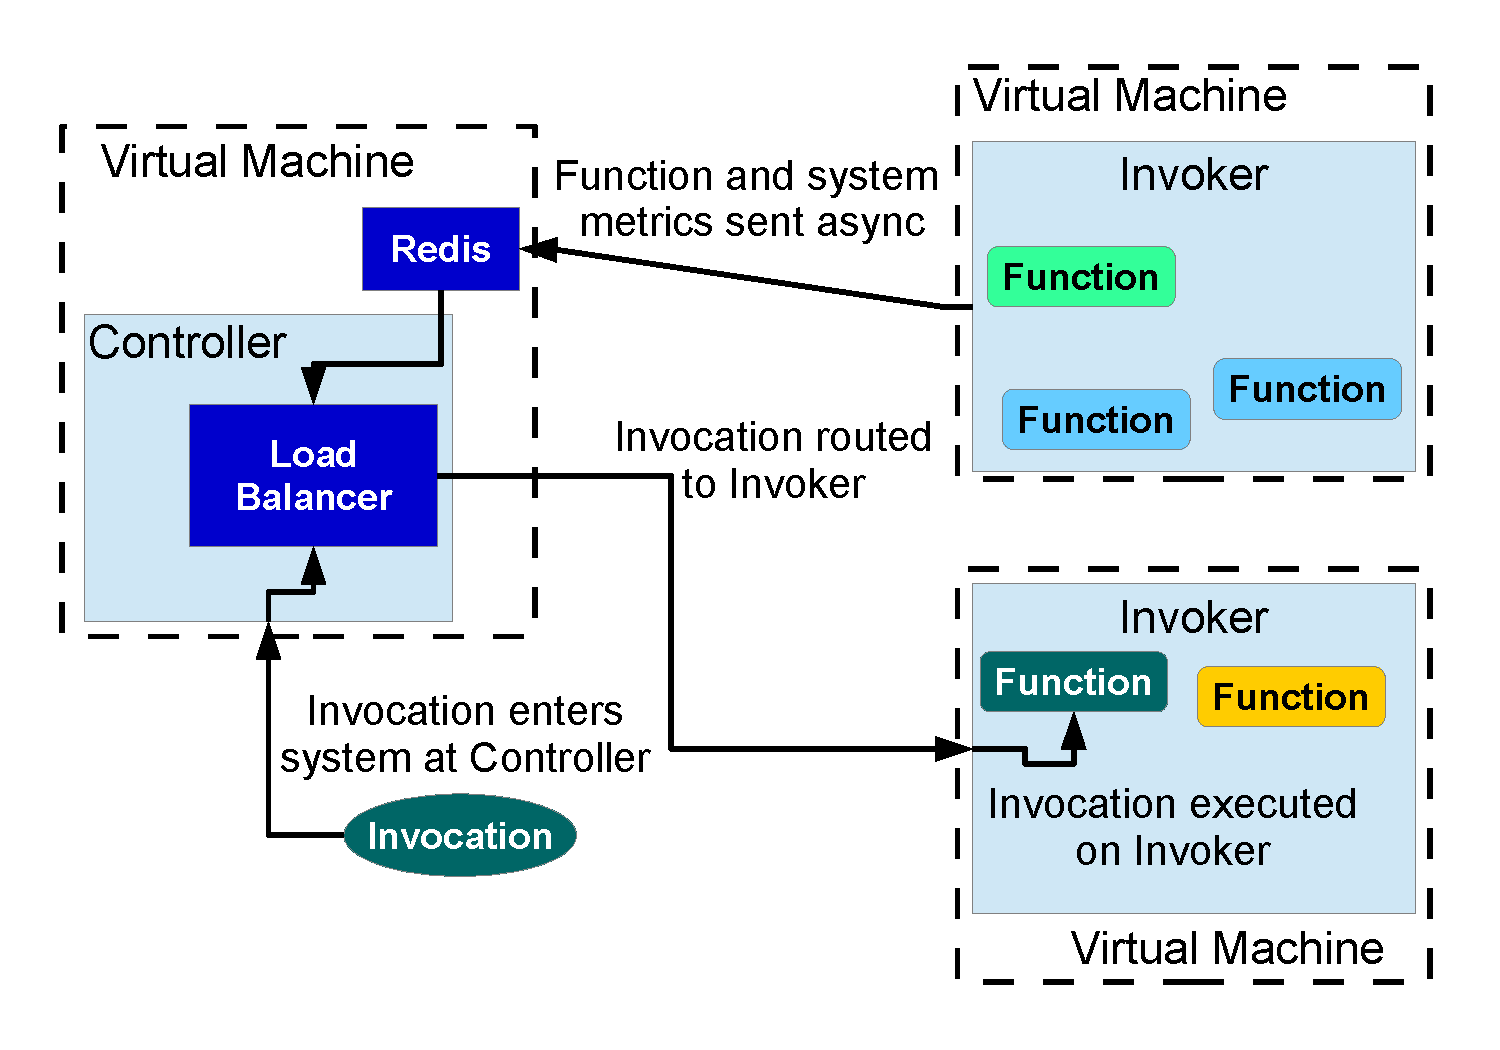
\includegraphics[width=0.7\textwidth]{chrlu/faaslb-osdi22/figs/sys-diag.pdf}
 %   \vspace*{-0.3cm}
  \caption{System diagram of relevant OpenWhisk components and communication used to schedule and run function invocations.}
  \label{fig:sys-diag}
  %  \vspace*{-0.3cm}
\end{figure}

The CH-RLU algorithm described in the previous section requires two main additional pieces of information from each invoker/server: the load averages, and the cold/warm running times of functions. 
Both of these are periodically (every 5 seconds) captured and stored in a centralized redis key-value store.
The load-balancer in the controller reads these asynchronously: working with stale and inconsistent metrics is our key design goal. 
The default load-bound, b, is 1.2, and the max load, b\_max is 6. Popularity threshold is set to 20\%.
We did not observe performance to be very sensitive to these parameters, and thus do not need to auto-tune them, and they are suitable as user-inputs. 

%\vspace*{-0.2cm}
\subsection{Performance Optimizations For OpenWhisk}

Since our goal is to run functions under high load, we ran into a large number of OpenWhisk performance and scalability bottlenecks.
We found default OpenWhisk to be almost unusably slow and unstable even under reasonable load. 
We present their details and our actions to overcome them, hoping that the fast-growing serverless computing research field can benefit from our lessons. 


In our experience, the primary source of scalability bottlenecks when concurrently managing Docker containers.
We found significant contention in \texttt{dockerd}, Docker's control daemon which handles all the container lifecycle events.
Even at moderate loads (normalized server load average close to 1), high dockerd contention can increase tail latencies by \emph{several minutes!}


Currently, OpenWhisk \textbf{pauses} each container after function execution, which prevents it from being scheduled by the CPU.
It then resumes the container before running the next invocation of the same function (assuming a warm start).
Each invocation therefore requires these two additional (pause/resume) events to be handled by dockerd, which results in significant lock contention.
Because of the FaaS programming model, the pausing is not necessary, since nothing in the container can run after a function has returned.
Therefore, we remove these redundant pause/resume operations to reduce dockerd contention.
This reduces the OpenWhisk overhead by 0.2 seconds \emph{per-invocation} on average.
More importantly, by reducing dockerd contention, we were able to run a much larger number of concurrent functions. 

An even larger source of scalability bottleneck is \textbf{network} namespace creation time.
Using the default bridge networking requires each invocation to create a new TUN/TAP network interface.
We found this to be a very expensive operation because of Linux network stack overheads (several 100 ms), and because of dockerd's userspace lock (futex) contention for its networking database. 
We found that as the \emph{historical} total number of containers launched grows, so does the size of the network-interface database.
Dockerd reads and updates this database under the critical section, and the larger database results in higher lock contention.
As a result, we were unable to use VMs/servers with more than 4 CPUs after 20 minutes of sustained load, since the dockerd contention resulted in many functions timing out (timeout was 5 minutes)! 

We sidestep this problem by not using bridge networking, but instead using Docker's \textit{host} network option and assigning each container a unique port on the host. 
Implementing the network change required updating the OpenWhisk runtimes used to wrap functions to monitor their specified port.
This change allowed us to run functions on larger invokers and under more sustained load, and eliminated most timeouts. 

Finally, after a certain request rate threshold, we found the default \texttt{nginx} OpenWhisk frontend would crash and return \textit{502 BAD GATEWAY} for all URLs. 
We did not discover the cause of this problem, and simply bypassed it by letting function invocations to communicate with the controller/load-balancer directly. 

\noindent \textbf{CPU limits.} 
OpenWhisk uses the \textit{-{}-cpu-shares} option to set container CPU priority.
This has an unintended consequence of allowing functions to use more than one CPU core while running.
Major FaaS providers constrain functions to a single core unless they have extremely high memory allocations (<1 GB).
In order to stay in line with providers and prevent outsized impact on system load from some functions, we use the \textit{-{}-cpus} flag instead to assign each function no more than one CPU.

Together, these performance optimizations have allowed us to run OpenWhisk on invokers that are $4\times$ larger, and serve more than $6\times$ the load, without dropping functions due to timeouts.
%
We plan to upstream all these performance optimizations in OpenWhisk to provide a higher-performance and lower-jitter control plane for FaaS research and production deployments. 

\begin{comment}
\noindent \textbf{docker pause.} 
OpenWhisk pauses Docker containers after each invocation completes to prevent the user code from continuing to run.
We disable this pausing because it causes significant contention inside Docker, affecting both latency and the ability to run more concurrent functions on an individual server.
Because we control the code running inside all our functions, we do not need the pausing as a security concern or to limit impact on load.
Our functions do not do anything outside of an invocation.

\noindent \textbf{configuration.}
While OpenWhisk provides a large number of configurable settings, most of them are locked into files.
In order to make the settings more amenable to prototyping and rapid changes, we converted many of them to also work as injectable environment variables.


\end{comment}



% SPACE: can be safely removed to get space back
% OPTIMIZATION
%Finding the consistent hash node a function hashes to is a relatively expensive operation, so we simply cache these pairs for fast lookup.
% Any time we change the hash ring (i.e. an invoker comes or goes) we simply empty the cache and allow it to refill as requests come along.


% SPACE: can be safely removed to get space back

% \begin{enumerate}
%   \item docker contention
%   \item host network
%   \item OW usage of docker CPU limits
%   \item general significant OW overhead
%   \item skip nginx
%   \item make many settings configurable
% \end{enumerate}

% OW Overhead median = 0.05472302436828605 seconds
% ShardingContainerPoolBalancer [0.0215673  0.05472302 0.86742063 4.59444914 6.49693995]
% quantiles: [0.1, 0.5, 0.8, 0.90, 0.99]
